The lack of quantitative knowledge about soot inception and surface growth pathways has hindered the development of accurate models for prediction of soot mass and morphology. The uncertainties in description gas chemistry for small and large intermediates could results in orders of magnitude difference in concentration of PAHs. The uncertainty is amplified through inception models making the soot modeling even more challenging. As a results, the choice of the reaction mechanism becomes a critical factor in soot modeling. A series of simulations were run using the CPR model of omnisoot without soot to highlight the difference between of six reaction mechanisms in description of gas chemistry during pyrolysis of $10\%$ $\mathrm{CH_4}$-Ar at $\mathrm{T_5}$=2200 K and $\mathrm{P_5}$=4.5 atm. The selected reaction mechanisms are: ABF~\citep{appel2000kinetic}, Caltech~\citep{blanquart2009chemical}, KAUST~\citep{wang2013pah}, CRECK~\citep{saggese2015kinetic}, ITV~\citep{hellmuth2024role}, NUIG~\citep{zhu2023wide}. These mechanisms have been widely used in flames and reactors. The last three mechanisms are actively being developed and tested recently. The comparison of mechanisms is based on the predicted carbon mass fraction (CMF) of species involved in soot formation. Here, carbon mass fraction is defined as the carbon mass in each species normalized by total carbon mass in the gas mixture which stays constant during the process in the absence of soot formation. The CMF of methane equals 1 at t=0 indicating that all carbon is initially stored in $\mathrm{CH_4}$ for the studied shock tube. It should be noted that the CRECK mechanism used in these simulations does not include "{BIN}`` species that represent the mass bins of soot particles.

Figure~\ref{fig:CH4_C2H4_A2R5_chem} shows the variability of CMF of $\mathrm{CH_4}$, $\mathrm{C_2H_2}$, and A2R5 predicted using different reaction mechanisms. The carbon mass fraction of $\mathrm{CH_4}$ provides a good measure of carbon flux from the fuel to the intermediate species. $\mathrm{C_2H_2}$ is the most abundant hydrocarbon during the pyrolysis and the key element in HACA scheme for growth of PAHs beyond benzene and surface growth of soot. Researchers has highlighted the importance of A2R5 in soot inception because of a low-aromaticity free edge can react readily with $\sigma$-radicals and form localized $\pi$-radicals (if partially hydrogenated), enabling combined covalent/stacked complexes~\citep{martin2019reactivity}. It can be seen in the inset of Figure~\ref{fig:CH4_C2H4_A2R5_chem}-a CRECK predicts a larger $\mathrm{CH_4}$ conversion up to 1 ms, but the trends changes for longer residence times where KAUST predicts the lowest CMF. ABF and NUIG underpredict methane conversion rate compared to the other mechanisms by nearly 10\% of the initial carbon. As expected, the majority (40-60\%) of the initial carbon is converted to $\mathrm{C_2H_2}$ by the end of the simulation. It can be seen in the inset of Figure~\ref{fig:CH4_C2H4_A2R5_chem}-b, the predictions of all they overall direct more carbon to $\mathrm{C_2H_2}$ at the end of 5 ms of the simulation. CRECK predicts a larger $\mathrm{C_2H_2}$ CMF up to 1 ms, and after than NUIG predicts the largest $\mathrm{C_2H_2}$ CMF that increases with time because this mechanism does not contain aromatics and large hydrocarbons so it does consider the conversion of $\mathrm{C_2H_2}$ to PAHs. The relative difference between the mechanisms is more pronounced for A2R5, spanning over an order of magnitude between ABF and Caltech. Since soot inception is described as the dimerization of PAHs, such differences are amplified with a one-order-of-magnitude variation in monomer concentration potentially leading to a two-order-of-magnitude difference in dimer formation. 
\begin{figure}[H]
	\centering
	\begin{subfigure}[t]{0.31\textwidth}
		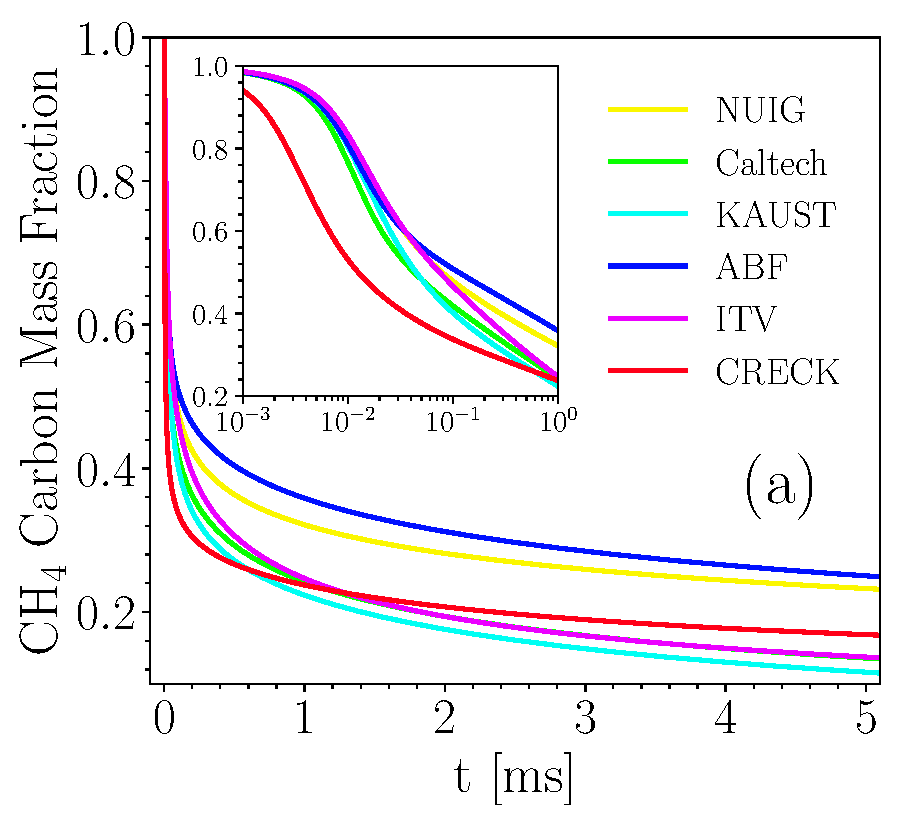
\includegraphics[width=1\textwidth]{Figures/Results/chemistry/CH4.pdf}
	\end{subfigure}
	\begin{subfigure}[t]{0.31\textwidth}
		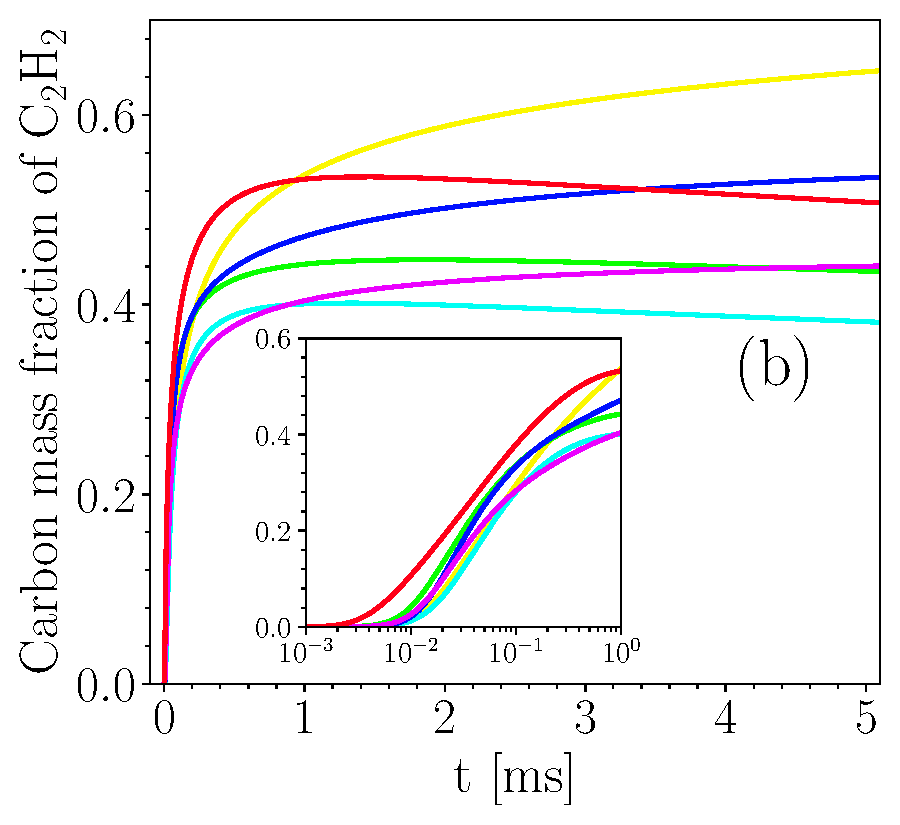
\includegraphics[width=1\textwidth]{Figures/Results/chemistry/C2H2.pdf}
	\end{subfigure}
	\begin{subfigure}[t]{0.31\textwidth}
		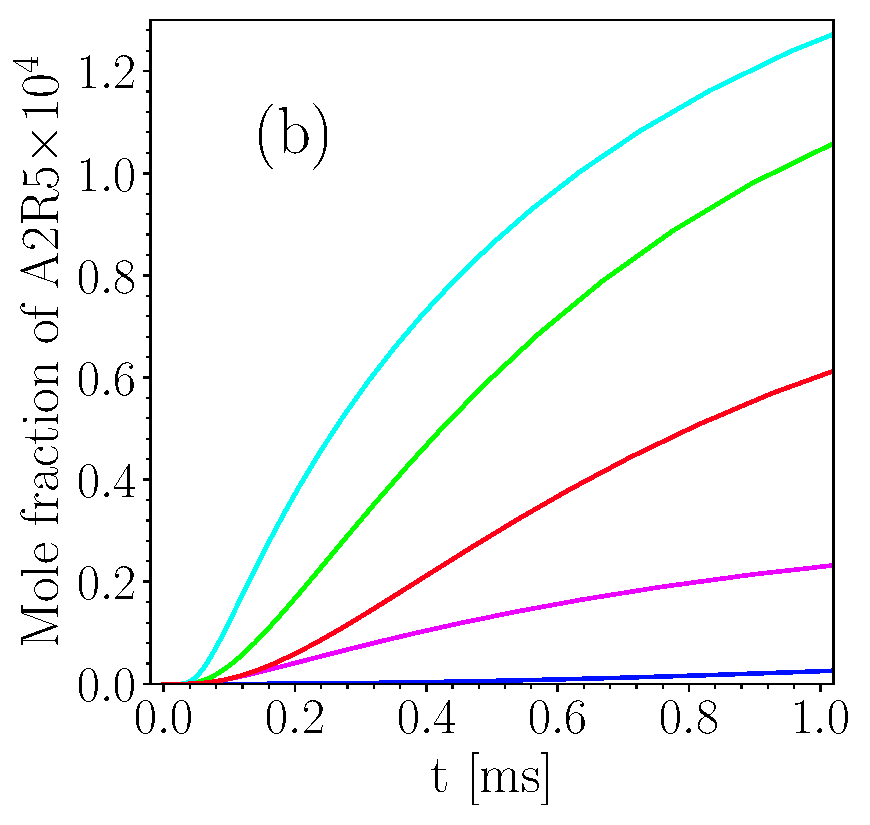
\includegraphics[width=1\textwidth]{Figures/Results/chemistry/A2R5.pdf}
	\end{subfigure}
	\caption{The carbon mass fraction of $\mathrm{CH_4}$ (a), $\mathrm{C_2H_2}$ (b), and A2R5 (c) at during pyrolysis of 10\%~$\mathrm{CH_4}$-Ar predicted using different reaction mechanisms. The insets provide a zoomed-in view of the early-time behavior}
	\label{fig:CH4_C2H4_A2R5_chem} 
\end{figure}

Omnisoot has the capability of loading all standard reaction mechanisms through Cantera, but the soot simulations in this work were conducted using Caltech and KAUST because they contain all the designated soot precursors and provide a high carbon flux to PAHs sufficient to predict soot yield and volume fraction close to the measurements. ITV mechansism also satisfies the criteria but the extensive size of the mechanism (species 759 and reactions 7582) significantly increases the computational cost of parametric studies and simulations.

%
%\begin{figure}[H]
%	\centering
%	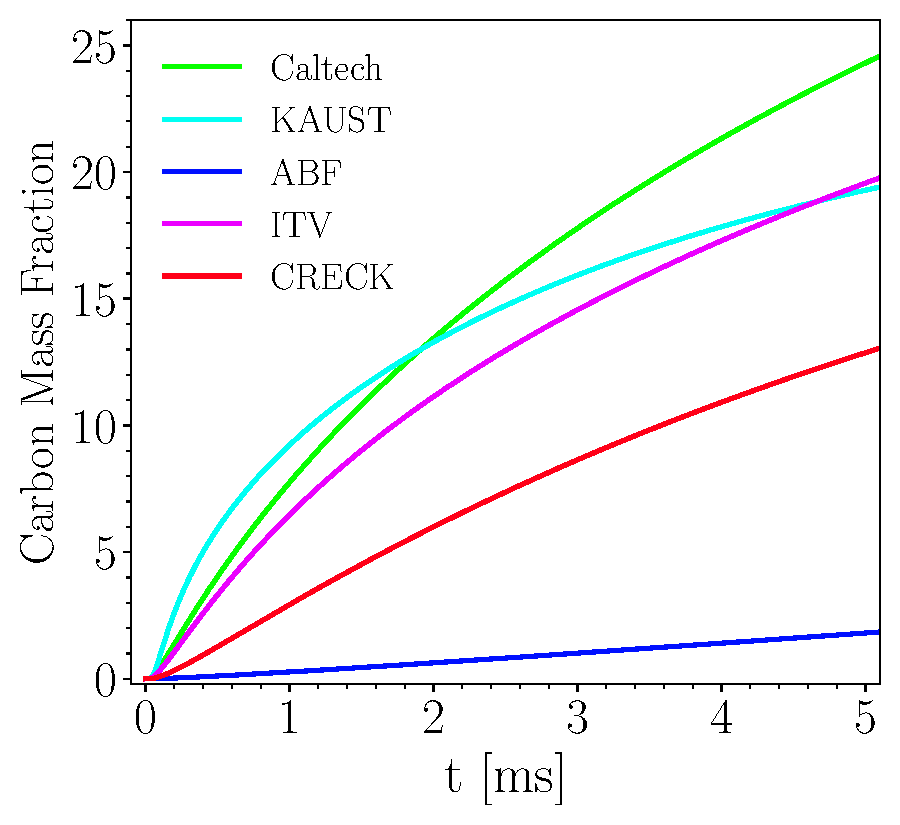
\includegraphics[width=0.32\textwidth]{Figures/Results/chemistry/med_hydrocarbons.pdf}
%	\caption{The carbon mass fraction of $\mathrm{C_{10}}$ to  $\mathrm{C_{18}}$ during pyrolysis of 10\%~$\mathrm{CH_4}$-Ar predicted using different reaction mechanisms}
%	\label{fig:PAHs_chem} 
%\end{figure}